\section{Materiales y datos}\label{sec:data}

\subsection{Área de estudio}

El área de estudio es la provincia de Cauquenes (región del Maule, Chile;
\ang{35.5}--\ang{36.3}~S, \ang{71.5}--\ang{73.3}~O), que comprende la
Cordillera de la Costa y el secano interior entre el océano Pacífico y el
valle central (figura~\ref{fig:area}). Su elevación en la grilla MODIS varía
entre \SI{0}{\metre} y \SI{\SceneElevMax}{\metre}. El uso del suelo combina
plantaciones forestales, matorral y pradera de secano, viñedos de secano y
cultivos de riego en los valles. En febrero, al final del verano seco
mediterráneo, la superficie presenta un contraste marcado entre vegetación
con acceso a agua y laderas secas, condición favorable para la calibración
interna de METRIC.


\begin{figure}[htbp]
\centering
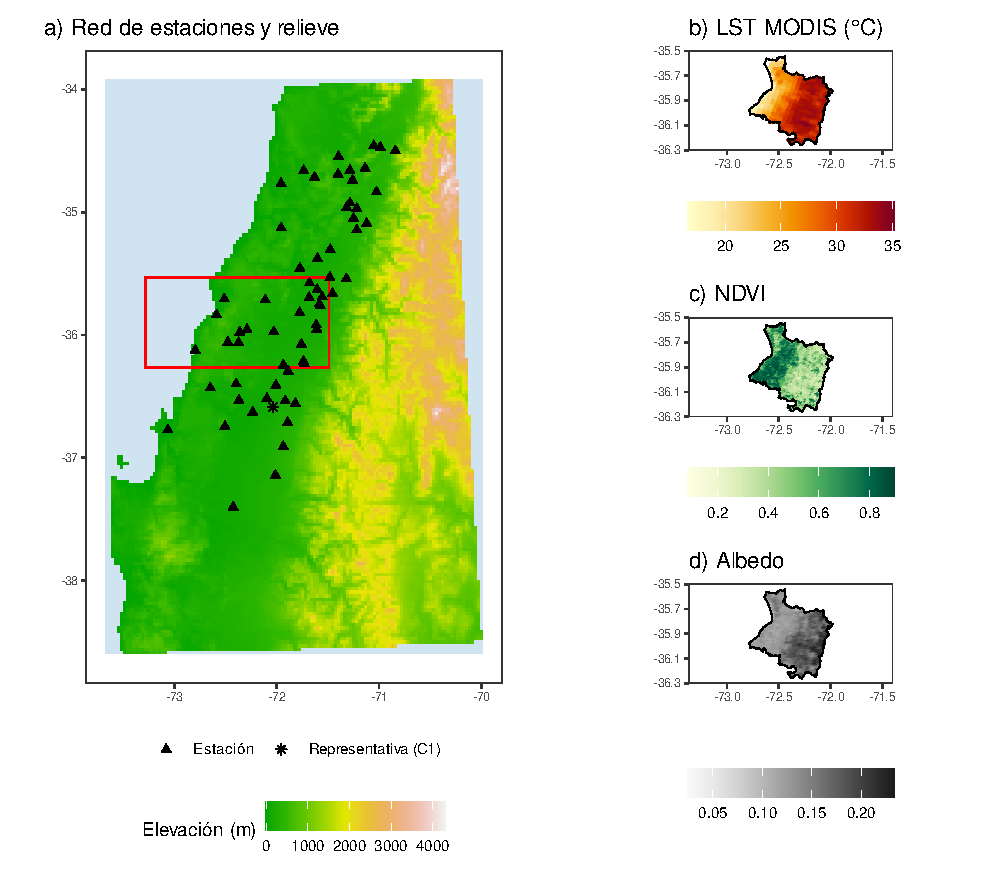
\includegraphics[width=\textwidth]{fig01_area.pdf}
\caption{(a) Red de estaciones meteorológicas sobre el relieve (Copernicus
GLO-90); el rectángulo rojo es la extensión de la escena y el asterisco la
estación representativa de C1. (b--d) Temperatura superficial, NDVI y albedo
MODIS del 15-02-2019 en la provincia de Cauquenes. Coordenadas geográficas
(WGS~84) solo para visualización.}\label{fig:area}
\end{figure}

\subsection{Observaciones satelitales}

Se usa la escena de ejemplo \code{cauquenes\_modis} de EarthFlux: el estado
de superficie MODIS colección~6.1 del 15 de febrero de 2019 (paso de Terra
cerca de las 14:08~UTC; nubosidad del mosaico h12v12 de 3~\%). Integra la
temperatura superficial diurna y las emisividades de las bandas 31--32 de
MOD11A1 \parencite{wan2021mod11a1,wan2014mod11c6}, el albedo de cielo blanco
de MCD43A3 \parencite{schaaf2021mcd43a3,schaaf2002brdf}, el NDVI de MOD13A2
\parencite{didan2021mod13a2} y el LAI de MCD15A2H
\parencite{myneni2021mcd15a2h}, en la grilla sinusoidal de
$\approx\SI{926,6}{\metre}$. La escena contiene \SceneCellsProvince
celdas dentro de la provincia, \SceneCellsValid
de ellas con todas las variables válidas. La procedencia de cada gránulo,
la máscara de calidad y las palabras de \emph{flags} se documentan en el
paquete. La elevación proviene del modelo Copernicus GLO-90, promediado a
cada celda.

\subsection{Observaciones meteorológicas}\label{sec:stations}

\StationDataText

Todas las estaciones se procesan con la tabla estándar y el control de
calidad de EarthFlux (\code{ef\_station\_table()}, \code{ef\_station\_qc()}),
que marca y nunca elimina en silencio. Las covariables de regionalización
son la elevación media de \SI{1}{\kilo\metre} (Copernicus GLO-90) y la
distancia a la costa (Natural Earth 1:10~m), en una grilla UTM~18S de
\SI{1}{\kilo\metre}. No se usan covariables derivadas de la superficie
(LST, NDVI) para evitar la circularidad entre la temperatura del aire
regionalizada y la temperatura superficial que gobierna la calibración de
$dT$ (decisión D-11).

\subsection{Referencias de validación}\label{sec:validation-data}

Se buscaron mediciones independientes de $\ETa$ o de flujo de calor latente
(covarianza de torbellinos, lisímetros) para la región y la fecha. La red
AmeriFlux registra cinco sitios en Chile, todos fuera del área (Chiloé,
Alerce Costero, Fray Jorge, Omora). Las torres de covarianza de torbellinos
operadas en viñedos y huertos de Talca y Ñuble
\parencite{carrascobenavides2014metric,ortegafarias2010twolayer} no tienen
datos públicos para febrero de 2019, y el único conjunto abierto cercano
encontrado (huertos de avellano en Ñuble, Zenodo) contiene salidas de un
modelo y no mediciones. Por lo tanto, \textbf{este estudio no dispone de
referencias independientes para validar la exactitud absoluta de $\ETa$}. La
validación se limita a las variables meteorológicas, para las que sí existen
observaciones independientes (validación cruzada espacial,
sección~\ref{sec:design}). Los reanálisis no se usan como verdad
observacional.

\section{Metodología}\label{sec:methods}

\subsection{Arquitectura de EarthFlux y niveles de evidencia}

EarthFlux (versión \EarthFluxVersion, commit \texttt{\EarthFluxCommit})
organiza la física de METRIC en funciones vectorizadas e independientes del
sensor (radiación, $G$, rugosidad, anclas, calibración de $H$, $LE$, $ET$),
un módulo de forzamiento meteorológico (tabla de estaciones, control de
calidad, ET de referencia FAO-56 y ASCE-EWRI) y un módulo de
regionalización con interfaz común para C1, C2 y C3 (\code{ef\_regionalize()},
\code{ef\_regionalize\_cv()}) y núcleo GWR propio verificado contra
\pkg{GWmodel} \parencite{gollini2015gwmodel}. Toda elección científica sin
fuente única carece de valor por defecto y queda registrada en la
procedencia; los valores físicamente anómalos se marcan con \emph{flags} y
no se truncan. El estudio se ejecuta exclusivamente con la API pública del
paquete, en un directorio separado de su código (\code{research/cedes2027/}).

Se distinguen cuatro niveles de evidencia (tabla~\ref{tab:verification}):
(1) \emph{verificación de ecuaciones}: contraste, término a término, de cada
formulación con su fuente primaria; (2) \emph{pruebas de software}:
pruebas unitarias, de invariantes y de integración ejecutadas en cada
\code{R CMD check}; (3) \emph{validación meteorológica}: error fuera de
muestra de las variables regionalizadas frente a estaciones no usadas en el
ajuste; y (4) \emph{validación de $\ETa$}: comparación con mediciones
independientes de flujos, no disponible en este estudio.

\subsection{Diseño experimental}\label{sec:design}

El estudio comprende tres experimentos (figura~\ref{fig:workflow}).

\begin{figure}[htbp]
\centering
\begin{tikzpicture}[node distance=4mm and 6mm, font=\footnotesize,
  box/.style={draw, rounded corners, align=center, fill=#1, minimum height=9mm, text width=3.1cm},
  box/.default=white, arr/.style={-{Stealth[length=2mm]}, thick}]
\node[box=gray!12] (st) {\NStations{} estaciones horarias\\(DMC, INIA, FDF, NOAA)};
\node[box=gray!12, below=of st] (dem) {Elevación y distancia\\a la costa (1 km)};
\node[box=gray!12, below=of dem] (modis) {Escena MODIS\\15-02-2019 (1 km)};
\node[box=teal!12, right=of st, yshift=-6.5mm] (reg) {Regionalización\\C1, C1-lap, C2-OLS,\\C2-IDW, C3-GWR};
\node[box=teal!12, right=of reg] (cv) {\textbf{Exp. R}: validación\\cruzada espacial\\anidada (90 días)};
\node[box=orange!15, below=of reg, yshift=-5mm] (metric) {METRIC: $R_n$, $G$, anclas,\\$r_{ah}$, $H$, $LE$, $\mathrm{ET_rF}$};
\node[box=orange!15, right=of metric] (m) {\textbf{Exp. M}: sustitución\\completa y de una\\variable por vez};
\node[box=orange!15, below=of m] (s) {\textbf{Exp. S}: Monte Carlo\\anclas, ruido MODIS,\\alternativas};
\node[box=gray!5, below=of metric] (eta) {$\mathrm{ET_a} = \mathrm{ET_rF}\cdot\mathrm{ET_r^{24}}$};
\draw[arr] (st) -- (reg); \draw[arr] (dem) -- (reg); \draw[arr] (reg) -- (cv);
\draw[arr] (reg) -- node[left, font=\scriptsize]{$T_a, e_a, u_2, \mathrm{ET_r}$} (metric);
\draw[arr] (modis) -- (metric); \draw[arr] (metric) -- (eta);
\draw[arr] (metric) -- (m); \draw[arr] (m) -- (s);
\end{tikzpicture}
\caption{Diseño del estudio. Los tres experimentos comparten estaciones,
covariables, escena, ecuaciones y criterios de calibración; solo cambia la
representación espacial del forzamiento meteorológico.}\label{fig:workflow}
\end{figure}


\paragraph{Experimento R: regionalización meteorológica.} Para cada hora
de paso (14:00~UTC) de los \NCVDays{} días entre el 1 de enero y el 31 de
marzo de 2019, y para la temperatura del aire, la presión de vapor y la
velocidad del viento a \SI{2}{\metre} (convertida desde la altura del
anemómetro con el perfil logarítmico de FAO-56), se evaluaron C1, C1-lap
(solo temperatura), C2-OLS, C2-IDW y C3-GWR mediante validación cruzada por
bloques espaciales de \SI{50}{\kilo\metre} (\NFolds{} pliegues). El ancho de
banda de GWR (núcleo bicuadrado, $k$ adaptativo, AICc) y la potencia de IDW
($p\in\{1,2,3\}$, LOOCV) se vuelven a seleccionar dentro de cada conjunto de
entrenamiento (validación anidada), de modo que ninguna estación de
evaluación interviene en la selección. La estación representativa de C1 se
eligió con una regla fijada antes de ver los errores (D-02): la estación
completa más cercana al centroide de la provincia. Las métricas son RMSE,
MAE, sesgo (predicho $-$ observado) y correlación de Pearson; sus intervalos
de confianza del 95~\% se obtuvieron por \emph{bootstrap} de bloques que
remuestrea días completos ($B=2000$), lo que conserva junta la dependencia
espacial de los errores de un mismo instante. La comparación con GWR se
hizo de forma pareada sobre las mismas predicciones fuera de muestra
(diferencia media de errores cuadráticos, $\Delta SE$).

\paragraph{Experimento M: propagación en METRIC.} Para el día de la escena
se regionalizaron las 24 horas locales (UTC$-3$) de las tres variables con
cada configuración, con las mismas estaciones, control de calidad,
covariables y horas; los vacíos horarios de hasta 6~h se rellenaron por
interpolación temporal y se contaron (D-09). Los campos se proyectaron a la
grilla MODIS. La $\ETr$ horaria de alfalfa (ASCE-EWRI) se calculó por píxel
a partir de los campos regionalizados y de la radiación de onda corta
modelada, igual para todas las configuraciones (D-04); $\ETr^{24}$ es la
suma de las 24 horas. METRIC se ejecutó con idénticas ecuaciones, máscaras,
insumos MODIS, criterios de anclas y condiciones de borde
(tabla~\ref{tab:options}). Las anclas se seleccionan solo con variables de
superficie (D-08) dentro de las celdas con todos los insumos válidos; si
el forzamiento es válido en toda la escena, las anclas son las mismas celdas
en todas las corridas (se verificó corrida por corrida), de modo que los
cambios de calibración se deben exclusivamente al forzamiento evaluado en
esas celdas. Se realizaron
dos tipos de corrida: (a) \emph{sustitución completa}, con cada
configuración; y (b) \emph{sustitución de una variable por vez}, partiendo de
C1 y reemplazando una sola entrada ($T_a$, $e_a$, $u_2$, $\ETr$ instantánea
o $\ETr^{24}$) por su campo C3-GWR. La comparación usa C1 como línea base
porque representa la práctica convencional, no porque se suponga correcta.


\begin{table}[htbp]
\centering\footnotesize
\caption{Opciones de METRIC comunes a todas las configuraciones (decisiones
del estudio; ver \texttt{docs/decisions.md}).}\label{tab:options}
\begin{tabularx}{\textwidth}{>{\raggedright\arraybackslash}p{4.3cm}>{\raggedright\arraybackslash}X>{\raggedright\arraybackslash}p{2.6cm}}
\toprule
Componente & Elección & Estado / decisión \\
\midrule
Onda corta incidente & Transmisividad particionada de Allen ($K_t = 1$), terreno plano & CANDIDATA \\
Flujo de calor del suelo & Bastiaanssen ($G/R_n$ en función de $T_s$, $\alpha$, NDVI) & VERIFICADA; D-05 \\
Rugosidad & $z_{om} = 0{,}018\,\mathrm{LAI}$, mínimo \SI{0,005}{\metre} & D-06 \\
Viento a la altura de mezcla & Perfil logarítmico desde \SI{2}{\metre}, $z_{om}$ de la estación \SI{0,015}{\metre}, $z_b = \SI{200}{\metre}$ & VERIFICADA \\
Estabilidad & Monin--Obukhov iterativa; $\psi_m$ estable a \SI{2}{\metre}; tolerancia 0,01; máx. 20 iteraciones & VERIFICADA; P0-10 \\
Anclas & Frías: NDVI $\ge P_{95}$ y 20\,\% más frío; calientes: NDVI $\le P_{10}$ y 20\,\% más cálido; mediana & CANDIDATA; D-08 \\
Condiciones de borde & $\mathrm{ET_rF}_{cold} = 1{,}05$; $LE_{hot} = 0$ & D-07 \\
Corrección de $T_s$ & $\Gamma = \SI{6,5}{\kelvin\per\kilo\metre}$ a la elevación mediana & VERIFICADA (forma) \\
Calor latente de vaporización & Constante, \SI{2,45}{\mega\joule\per\kilo\gram} & P0-7 \\
ET de referencia & Alfalfa, ASCE-EWRI horaria; $\mathrm{ET_r^{24}}$ = suma de 24 horas & VERIFICADA; D-04 \\
\bottomrule
\end{tabularx}
\end{table}

\paragraph{Experimento S: sensibilidad y robustez.} Con los forzamientos C1
y C3-GWR (o la mejor alternativa espacial factible) se realizaron
\NMC{} réplicas Monte Carlo de (S-A) los criterios de anclas y las
condiciones de borde (percentil de NDVI frío $\sim U(0{,}90;0{,}98)$, caliente
$\sim U(0{,}05;0{,}20)$, fracciones seleccionadas $\sim U(0{,}1;0{,}3)$,
$\ETrF_{cold}\sim U(1{,}00;1{,}10)$) y de (S-B) los insumos MODIS (LST con
ruido $N(0,\SI{1}{\kelvin})$ por píxel más un sesgo de escena
$N(0,\SI{0,5}{\kelvin})$, coherente con la exactitud de MOD11
\parencite{wan2014mod11c6}; albedo con error relativo $N(0;0{,}05)$), además
de (S-C) alternativas estructurales deterministas (G de Bastiaanssen frente
a Tasumi, piso de rugosidad, agregación de anclas). En S-A y S-B, la misma
perturbación se aplica a ambos forzamientos, lo que permite estimar el
efecto del forzamiento de forma pareada y compararlo con la dispersión
inducida por las otras fuentes. Con \NMC{} réplicas, el error estándar
Monte Carlo de una media es la desviación estándar dividida por
$\sqrt{\NMC}$, suficiente para las diferencias de interés.

\subsection{Reproducibilidad}

Los scripts del estudio (\code{research/cedes2027/scripts/}) descargan los
datos de fuentes públicas, registran sumas de verificación, fijan la
semilla (\num[group-separator={}]{\Seed}) y generan cada tabla, figura y
cifra del texto. Las cifras de este manuscrito se insertan desde un
archivo de macros generado a partir de las tablas de resultados, y cada una
está trazada a su archivo y procedimiento en el registro de afirmaciones
cuantitativas del material suplementario.
